\input preamble.tex
\Huge Prøve 01  i ultralydtransmitter 
\normalsize

\vskip 5pt 
Kompetansemål:
\begin{itemize}[noitemsep]
	%\item utføre arbeid på automatiserte anlegg fagmessig, nøyaktig og i overensstemmelse med krav til helse, miljø og sikkerhet og rutiner for kvalitetssikring og internkontroll
	%\item utføre risikovurdering og vurdere tiltak for ivaretakelse av person– og maskinsikkerhet
	%\item vurdere hvilke regelverk og normer som gjelder for arbeidet som skal utføres og anvende dette
	%\item planlegge, utføre, vurdere kvalitet, sluttkontrollere og dokumentere arbeidet
\item planlegge, programmere, montere og idriftsette programmerbare styresystemer
\item endre og tilpasse skjermbilder for grensesnitt mellom menneske og maskin
	%\item anvende ulike elektroniske kommunikasjonssystemer i automatiserte anlegg
	%\item vurdere datasikkerhet i automatiserte anlegg
	%\item tegne, lese og forklare instrumenterte prosessflytskjemaer og bruke annen relevant dokumentasjon for automatiserte anlegg
\item montere, konfigurere, kalibrere og idriftsettelse digitale og analoge målesystemer
	%\item idriftsette og optimalisere regulatorer basert på prosessbehov
	%\item montere og idriftsette ulike typer pådragsorganer med tilhørende forstillingselementer og hjelpeutstyr
	%\item programmere, idriftsette samt gjøre rede for roboters funksjon og anvendelse i produksjonsanlegg
	%\item måle fysiske størrelser i automatiserte anlegg
	%\item feilsøke og rette feil i automatiserte anlegg
	%\item bruke gjeldende regelverk og normer for elektriske installasjoner på maskiner
	%\item bruke gjeldende regelverk og normer for installasjon av elektroniske kommunikasjonssystemer
	%\item beskrive ulike vedlikeholdssystemer og -rutiner knyttet til automatiserte anlegg, og anvende et av disse
	%\item redegjøre for bedriftens organisasjonsoppbygging og bedriftens verdiskapning i et samfunnsperspektiv
	%\item dokumentere egen opplæring i automatiseringssystemer
\end{itemize}

Alle ark som leveres inn skal ha elevens navn. \\ 

Oppgave 1-8 skal leveres på papir, etter levering kan eleven ta frem PC og svare på oppgave 9.\\

\vskip 2.5pt 

\hrule
\vfil \eject
Oppgave 1 (6p)%Navngi
\vskip 2.5pt 
Hva viser dette bildet?
$$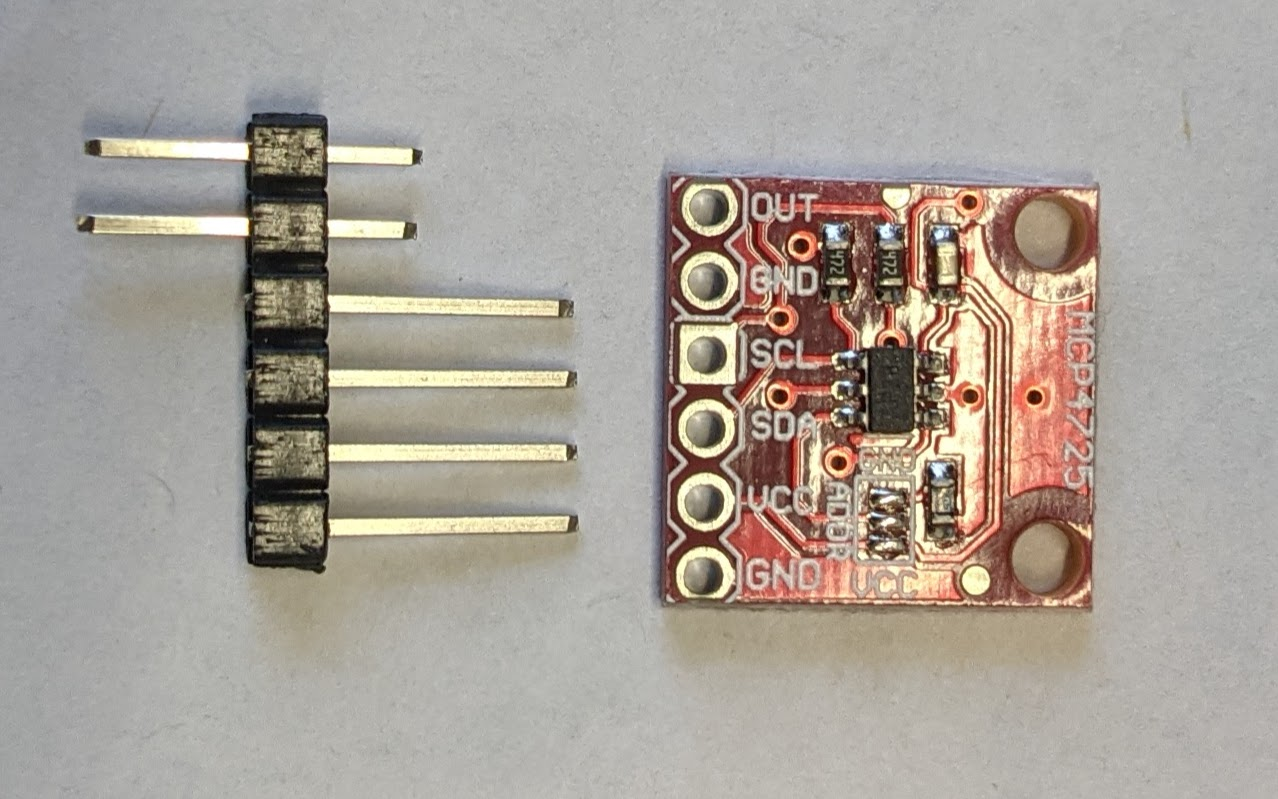
\includegraphics[width=8cm]{./lUltralydtransmitter0302.jpg}$$
\vskip 2.5pt 

\begin{tikzpicture}
	\draw[step=0.5cm,gray!20,very thin]  grid (17,4) ;
\end{tikzpicture}
\vskip 2.5pt 

Oppgave 2 (6p) %Definisjoner
\vskip 2.5pt 
Hva viser dette bildet?
$$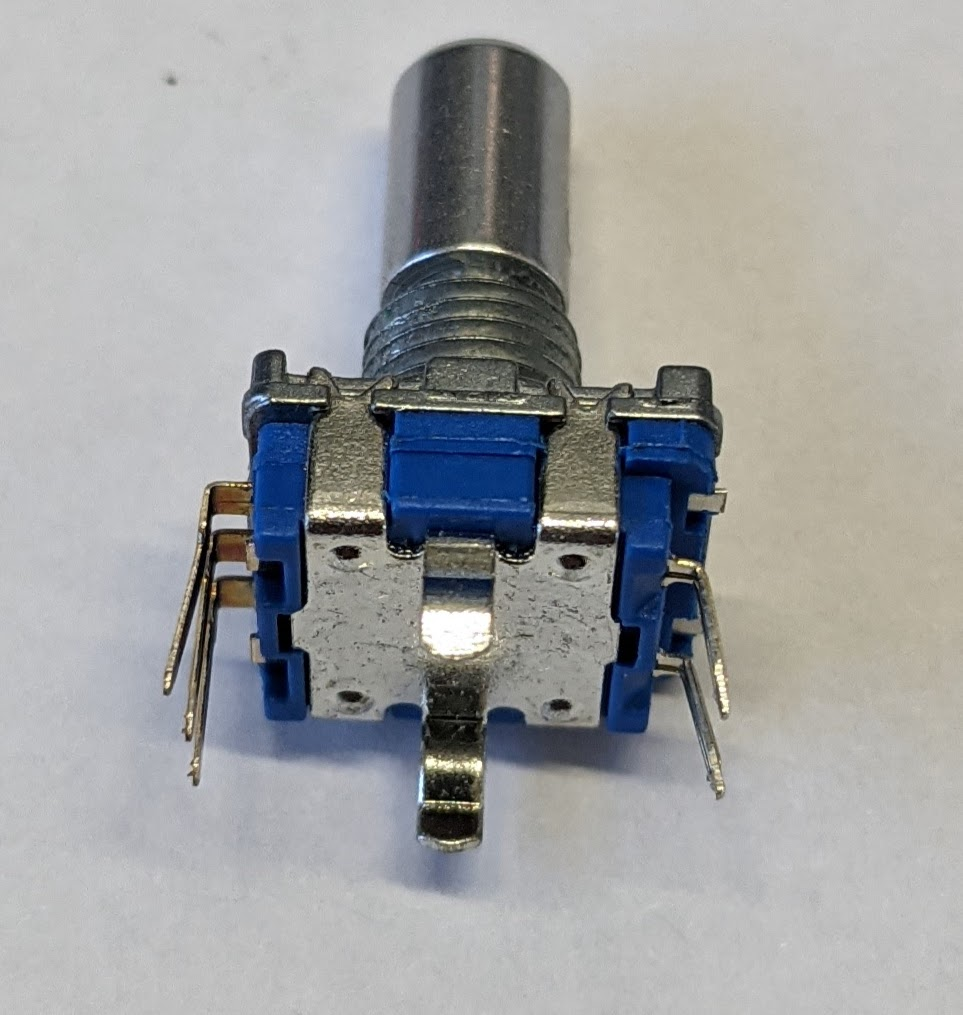
\includegraphics[width=8cm]{./lUltralydtransmitterx0501.jpg}$$
\vskip 2.5pt 

\begin{tikzpicture}
	\draw[step=0.5cm,gray!20,very thin]  grid (17,4) ;
\end{tikzpicture}
\vskip 2.5pt 

Oppgave 3 (6p)%Enkel utregninger.
\vskip 2.5pt 
Du skal måle en distanse fra 0-0.75 m vis hvordan du kan skallere dette til bruk mot en DAC på 12 bit. Det vil si at den har verdier fra 0 til og med 4095. 
\vskip 2.5pt 

\begin{tikzpicture}
	\draw[step=0.5cm,gray!20,very thin]  grid (17,8) ;
\end{tikzpicture}
\vskip 2.5pt 
Oppgave 4 (6p)
\vskip 2.5pt 
Hva menes med ultralyd?
\vskip 2.5pt 

\begin{tikzpicture}
	\draw[step=0.5cm,gray!20,very thin]  grid (17,4) ;
\end{tikzpicture}
\vskip 2.5pt 
\vfil \eject
Oppgave 5 (6p) %Feilsøkings oppgave

\vskip 2.5pt 
Tegn i hvordan  A og B pulsene vil se ut når slideren beveges som vist på bilde. 
$$\includegraphics[width=17cm]{./aUltralystransmitterx02.eps}$$
\vskip 2.5pt 
\vskip 2.5pt 
\vfil \eject
Oppgave 6 (6p) % Tegn og forklar virkemåte
\vskip 2.5pt 
Skriv på kommentarer som beskriver hva denne koden gjør. 
\begin{lstlisting}[language=Arduino]


const int trigger = 11;
const int echo = 10;

void setup()
{



	pinMode(trigger,OUTPUT);
	pinMode(echo,INPUT);
}
void loop()
{



	digitalWrite(trigger, LOW);
	delayMicroseconds(2);


	digitalWrite(trigger, HIGH);
	delayMicroseconds(10);
	digitalWrite(trigger, LOW);
	

	long duration = pulseIn(echo, HIGH);
	

	float distance = duration * 0.0343 / 2;
}
\end{lstlisting}
\vfil \eject

Oppgave 7 (6p) % Tegn og forkalr virkemåte. 
\vskip 2.5pt 
Skriv på kommentarer som beskriver hva denne koden gjør. 
\vskip 10pt 
\begin{lstlisting}[language=Arduino]


display.clearDisplay();


display.setTextSize(1);


display.setTextColor(SSD1306_WHITE);


display.setCursor(0,0);



display.print("Avstand = ");
display.print(distance);
display.print(" cm");



display.display(); 
\end{lstlisting}
\vfil \eject
Oppgave 8 (6p)
\vskip 2.5pt 
Tegningen viser de komponentene du har brukt i prosjektet deres. Tegn inn koblingene som er nødvendige for å få det til å virke. 
$$\includegraphics[width=9cm]{aUltralydtransmitterx01.eps}$$
\vskip 2.5pt 

\begin{tikzpicture}
	\draw[step=0.5cm,gray!20,very thin]  grid (17,4) ;
\end{tikzpicture}
\vskip 2.5pt 
\vskip 2.5pt 
%Oppgave 9 skal beskrive hvordan en jobb skal utføres. (Planlegg, besriv hvordan du vAlle gjenomført og dokumenter jobben)

\newpage
\
\newpage
Oppgave 9 (12p)

\vskip 5pt 

I denne oppgaven skal du modifisere programmet som dere har laget til deres ultralydtransmitter slik at følgende vises i displayet. 
\vskip 10pt 

Gruppe X\\
Nivaet i tanken \\
xx.xx m\\


\vskip 5pt 
Legg merke til at det står meter. Det vil si at du må modifisere slik at det stemmer. 
\end {document}
